% Options for packages loaded elsewhere
\PassOptionsToPackage{unicode}{hyperref}
\PassOptionsToPackage{hyphens}{url}
%
\documentclass[
  letterpaper,
  ignorenonframetext,
  aspectratio=43,
  handout,
  12pt]{beamer}
\usepackage{pgfpages}
\setbeamertemplate{caption}[numbered]
\setbeamertemplate{caption label separator}{: }
\setbeamercolor{caption name}{fg=normal text.fg}
\beamertemplatenavigationsymbolsempty
% Prevent slide breaks in the middle of a paragraph
\widowpenalties 1 10000
\raggedbottom
\setbeamertemplate{part page}{
  \centering
  \begin{beamercolorbox}[sep=16pt,center]{part title}
    \usebeamerfont{part title}\insertpart\par
  \end{beamercolorbox}
}
\setbeamertemplate{section page}{
  \centering
  \begin{beamercolorbox}[sep=12pt,center]{part title}
    \usebeamerfont{section title}\insertsection\par
  \end{beamercolorbox}
}
\setbeamertemplate{subsection page}{
  \centering
  \begin{beamercolorbox}[sep=8pt,center]{part title}
    \usebeamerfont{subsection title}\insertsubsection\par
  \end{beamercolorbox}
}
\AtBeginPart{
  \frame{\partpage}
}
\AtBeginSection{
  \ifbibliography
  \else
    \frame{\sectionpage}
  \fi
}
\AtBeginSubsection{
  \frame{\subsectionpage}
}
\usepackage{amsmath,amssymb}
\usepackage{lmodern}
\usepackage{iftex}
\ifPDFTeX
  \usepackage[T1]{fontenc}
  \usepackage[utf8]{inputenc}
  \usepackage{textcomp} % provide euro and other symbols
\else % if luatex or xetex
  \usepackage{unicode-math}
  \defaultfontfeatures{Scale=MatchLowercase}
  \defaultfontfeatures[\rmfamily]{Ligatures=TeX,Scale=1}
\fi
\usetheme[]{metropolis}
% Use upquote if available, for straight quotes in verbatim environments
\IfFileExists{upquote.sty}{\usepackage{upquote}}{}
\IfFileExists{microtype.sty}{% use microtype if available
  \usepackage[]{microtype}
  \UseMicrotypeSet[protrusion]{basicmath} % disable protrusion for tt fonts
}{}
\makeatletter
\@ifundefined{KOMAClassName}{% if non-KOMA class
  \IfFileExists{parskip.sty}{%
    \usepackage{parskip}
  }{% else
    \setlength{\parindent}{0pt}
    \setlength{\parskip}{6pt plus 2pt minus 1pt}}
}{% if KOMA class
  \KOMAoptions{parskip=half}}
\makeatother
\usepackage{xcolor}
\IfFileExists{xurl.sty}{\usepackage{xurl}}{} % add URL line breaks if available
\IfFileExists{bookmark.sty}{\usepackage{bookmark}}{\usepackage{hyperref}}
\hypersetup{
  hidelinks,
  pdfcreator={LaTeX via pandoc}}
\urlstyle{same} % disable monospaced font for URLs
\newif\ifbibliography
\usepackage{graphicx}
\makeatletter
\def\maxwidth{\ifdim\Gin@nat@width>\linewidth\linewidth\else\Gin@nat@width\fi}
\def\maxheight{\ifdim\Gin@nat@height>\textheight\textheight\else\Gin@nat@height\fi}
\makeatother
% Scale images if necessary, so that they will not overflow the page
% margins by default, and it is still possible to overwrite the defaults
% using explicit options in \includegraphics[width, height, ...]{}
\setkeys{Gin}{width=\maxwidth,height=\maxheight,keepaspectratio}
% Set default figure placement to htbp
\makeatletter
\def\fps@figure{htbp}
\makeatother
% Make links footnotes instead of hotlinks:
\DeclareRobustCommand{\href}[2]{#2\footnote{\url{#1}}}
\setlength{\emergencystretch}{3em} % prevent overfull lines
\providecommand{\tightlist}{%
  \setlength{\itemsep}{0pt}\setlength{\parskip}{0pt}}
\setcounter{secnumdepth}{-\maxdimen} % remove section numbering
\usepackage{pgfpages}
\pgfpagesuselayout{2 on 1}
\providecommand{\tightlist}{%
\setlength{\itemsep}{0pt}\setlength{\parskip}{0pt}}
\makeatletter
\makeatother
\let\Oldincludegraphics\includegraphics
\renewcommand{\includegraphics}[2][]{\Oldincludegraphics[width=\textwidth,height=0.7\textheight,keepaspectratio]{#2}}
\ifLuaTeX
  \usepackage{selnolig}  % disable illegal ligatures
\fi

\author{}
\date{}

\begin{document}

\hypertarget{ae731}{%
\section{AE731}\label{ae731}}

\begin{frame}{Theory of Elasticity}
\protect\hypertarget{theory-of-elasticity}{}
Dr.~Nicholas Smith

Wichita State University, Department of Aerospace Engineering August 19,
2021
\end{frame}

\begin{frame}{upcoming schedule}
\protect\hypertarget{upcoming-schedule}{}
\begin{itemize}
\tightlist
\item
  Aug 19 - Coordinate Transformation
\item
  Aug 24 - Principal Values
\item
  Aug 26 - Tensor Calculus
\item
  Aug 27 - Homework 1 Due
\item
  Aug 31 - Displacement and Strain
\end{itemize}
\end{frame}

\begin{frame}{outline}
\protect\hypertarget{outline}{}
\begin{itemize}
\tightlist
\item
  review
\item
  examples
\item
  index notation algebra
\item
  group problems
\item
  coordinate transformation
\item
  examples
\end{itemize}
\end{frame}

\hypertarget{review}{%
\section{review}\label{review}}

\begin{frame}{office hours}
\protect\hypertarget{office-hours}{}
\begin{itemize}
\tightlist
\item
  Homework will generally be due on Fridays
\item
  Feel free to e-mail me for an appointment outside office hours if the
  time does not work for you
\end{itemize}
\end{frame}

\begin{frame}{homework}
\protect\hypertarget{homework}{}
\begin{itemize}
\tightlist
\item
  Homework 1 is available on Blackboard if you want to start working on
  it
\item
  Covers all of Chapter 1, relatively difficult, don't wait until last
  minute
\item
  Study groups help a lot (but submit your own work)
\end{itemize}
\end{frame}

\begin{frame}{index notation}
\protect\hypertarget{index-notation}{}
Free index vs.~dummy index

\begin{columns}[T]
\begin{column}{0.5\textwidth}
\begin{itemize}
\tightlist
\item
  is not repeated on any term
\item
  takes all values (1,2,3)
\item
  e.g.~\(u_i = (u_1, u_2, u_3)\)
\item
  must match across terms in an express or equation
\end{itemize}
\end{column}

\begin{column}{0.5\textwidth}
\begin{itemize}
\tightlist
\item
  is repeated on at least one term
\item
  indicates summation over all values
\item
  e.g.~\(\sigma_{ii} = \sigma_{11} + \sigma_{22} + \sigma_{33}\)
\item
  can not be used more than twice in the same term
  (\(A_{ij}B_{jk}C_{kl}\) is good, \(A_{ij}B_{ij}C_{ij}\) is not)
\end{itemize}
\end{column}
\end{columns}
\end{frame}

\begin{frame}{symmetry}
\protect\hypertarget{symmetry}{}
\begin{itemize}
\item
  We can break any tensor up into symmetric and anti-symmetric portions
\item
  \(a_{ij} = \frac{1}{2} (a_{ij} + a_{ji}) + \frac{1}{2} (a_{ij} - a_{ji})\)
\end{itemize}
\end{frame}

\begin{frame}{example}
\protect\hypertarget{example}{}
\begin{itemize}
\tightlist
\item
  Find symmetric and anti-symmetric portions of
\end{itemize}

\[\begin{bmatrix}
1 & 4 & 3\\
2 & 1 & 5\\
4 & 3 & 6
\end{bmatrix}\]
\end{frame}

\begin{frame}{example symmetric portion}
\protect\hypertarget{example-symmetric-portion}{}
\[a_{(ij)} = \frac{1}{2}(a_{ij} + a_{ji})\]

\[a_{(ij)} = \frac{1}{2} \left (
\begin{bmatrix}
1 & 4 & 3\\
2 & 1 & 5\\
4 & 3 & 6
\end{bmatrix}+
\begin{bmatrix}
1 & 2 & 4\\
4 & 1 & 3\\
3 & 5 & 6
\end{bmatrix}\right)
= \begin{bmatrix}
1 & 3 & 3.5\\
3 & 1 & 4\\
3.5 & 4 & 6
\end{bmatrix}\]
\end{frame}

\begin{frame}{example anti-symmetric portion}
\protect\hypertarget{example-anti-symmetric-portion}{}
\[a_{(ij)} = \frac{1}{2}(a_{ij} - a_{ji})\]

\[a_{(ij)} = \frac{1}{2} \left (
\begin{bmatrix}
1 & 4 & 3\\
2 & 1 & 5\\
4 & 3 & 6
\end{bmatrix}-
\begin{bmatrix}
1 & 2 & 4\\
4 & 1 & 3\\
3 & 5 & 6
\end{bmatrix}\right)
= \begin{bmatrix}
0 & 1 & -0.5\\
-1 & 0 & 1\\
0.5 & -1 & 0
\end{bmatrix}\]
\end{frame}

\begin{frame}{special symbols}
\protect\hypertarget{special-symbols}{}
\begin{itemize}
\tightlist
\item
  For convenience we define two symbols in index notation
\item
  \emph{Kronecker delta} is a general tensor form of the Identity Matrix
\end{itemize}

\[\delta_{ij} = \left\{
\begin{array}{ll}
1& \text{if $i=j$}\\
0& \text{otherwise}
\end{array}
\right. = \begin{bmatrix}
1 & 0 & 0\\
0 & 1 & 0 \\
0 & 0 & 1
\end{bmatrix}\]

\begin{itemize}
\tightlist
\item
  Is also used for higher order tensors
\end{itemize}
\end{frame}

\begin{frame}{Kronecker delta}
\protect\hypertarget{kronecker-delta}{}
\begin{itemize}
\tightlist
\item
  \(\delta_{ij} = \delta_{ji}\)
\item
  \(\delta_{ij} = 3\)
\item
  \(\delta_{ij} a_j = a_i\)
\item
  \(\delta_{ij}a_{ij} = a_{ii}\)
\end{itemize}
\end{frame}

\begin{frame}{partial derivative}
\protect\hypertarget{partial-derivative}{}
\begin{itemize}
\tightlist
\item
  We indicate (partial) derivatives using a comma
\item
  In three dimensions, we take the partial derivative with respect to
  each variable \((x, y, z)\) or \((x_1, x_2, x_3)\)
\item
  For example a scalar property, such as density, can have a different
  value at any point in space
\item
  \(\rho = \rho(x_1, x_2, x_3)\)
\end{itemize}

\[\rho_{,i} = \frac{\partial}{\partial x_i} \rho = \left\langle \frac{\partial \rho }{\partial x_1}, \frac{\partial \rho }{\partial x_2}, \frac{\partial \rho }{\partial x_3} \right\rangle\]
\end{frame}

\begin{frame}{partial derivative}
\protect\hypertarget{partial-derivative-1}{}
\begin{itemize}
\tightlist
\item
  Similarly, if we take the partial derivative of a vector, it produces
  a matrix
\end{itemize}

\[u_{i,j} = \frac{\partial}{\partial x_j} u_i = \begin{bmatrix}
\frac{\partial u_1}{\partial x_1} & \frac{\partial u_1}{\partial x_2} & \frac{\partial u_1}{\partial x_3}\\
\frac{\partial u_2}{\partial x_1} & \frac{\partial u_2}{\partial x_2} & \frac{\partial u_2}{\partial x_3}\\
\frac{\partial u_3}{\partial x_1} & \frac{\partial u_3}{\partial x_2} & \frac{\partial u_3}{\partial x_3}
\end{bmatrix}\]
\end{frame}

\hypertarget{index-notation-algebra}{%
\section{index notation algebra}\label{index-notation-algebra}}

\begin{frame}{substitution}
\protect\hypertarget{substitution}{}
\begin{itemize}
\tightlist
\item
  When solving tensor equations, we often need to manipulate expressions
\item
  We need to make sure the correct indexes are used when substituting,
  for example
\item
  \(a_i = U_{im}b_m\)
\item
  \(b_i = V_{im}c_m\)
\item
  To substitute the second into the first, we need to change indexes
\end{itemize}
\end{frame}

\begin{frame}{substitution}
\protect\hypertarget{substitution-1}{}
\begin{itemize}
\tightlist
\item
  We need to change the free index, \emph{i}, to \emph{m} in the second
  equation
\item
  Since \emph{m} is already used as the dummy index, we need to change
  that too
\item
  \(b_m = V_{mj}c_j\)
\item
  We can now make the substitution
\item
  \(a_i = U_{im} V_{mj}c_j\)
\end{itemize}
\end{frame}

\begin{frame}{multiplication}
\protect\hypertarget{multiplication}{}
\begin{itemize}
\tightlist
\item
  We need to be careful with indexes when multiplying expressions
\item
  \(p = a_m b_m\) and \(q = c_m d_m\)
\item
  We can express, \emph{pq}, but remember the dummy index cannot be
  repeated more than once
\item
  \(pq \ne a_m b_m c_m d_m\)
\item
  Instead we must change the dummy index in one of the expressions first
\item
  \(pq = a_m b_m c_n d_n\)
\end{itemize}
\end{frame}

\begin{frame}{factoring}
\protect\hypertarget{factoring}{}
\begin{itemize}
\tightlist
\item
  In the following expression, we would like to factor out \emph{n}, but
  it has different indexes
\item
  \(T_{ij}n_j - \lambda n_i = 0\)
\item
  Recall \(\delta_{ij}a_j = a_i\), we can rewrite
  \(n_i = \delta_{ij}n_j\)
\item
  \(T_{ij}n_j = \lambda \delta_{ij}n_j = 0\)
\item
  \(T_{ij} - \lambda \delta_{ji})n_j = 0\)
\end{itemize}
\end{frame}

\begin{frame}{contraction}
\protect\hypertarget{contraction}{}
\begin{itemize}
\tightlist
\item
  \(T_{ii}\) is the contraction of \(T_{ij}\)
\item
  This can often be a useful tool in solving tensor equations
\item
  \(T_{ij} = \lambda \Delta \delta_{ij} + 2\mu E_{ij}\)
\item
  \(T_{ii} = \lambda \Delta \delta_{ii} + 2\mu E_{ii}\)
\end{itemize}
\end{frame}

\begin{frame}{example}
\protect\hypertarget{example-1}{}
\begin{itemize}
\tightlist
\item
  Solve the equation below for \(U_k\) in terms of \(P_i\) and \(a_i\).
  \[\mu \left[ \delta_{kj} a_i a_i + \frac{1}{1-2\nu} a_k a_j \right] U_k = P_j\]
  Multiply both sides by \(a_j\)
  \[\mu \left[ a_j \delta_{kj} a_i a_i + \frac{1}{1-2\nu} a_k a_j a_j \right] U_k = P_j a_j\]
  The dummy indexes can be changed
  \[\mu \left[ a_j \delta_{kj} a_i a_i + \frac{1}{1-2\nu} a_k a_i a_i \right] U_k = P_j a_j\]
\end{itemize}
\end{frame}

\begin{frame}{example}
\protect\hypertarget{example-2}{}
\begin{itemize}
\tightlist
\item
  \(a_j \delta_{kj} = a_k\)
  \[\mu U_k \left[ a_k a_i a_i + \frac{1}{1-2\nu} a_k a_i a_i \right] = P_j a_j\]
  Factoring
  \[\mu U_k a_k a_i a_i \left[ 1 + \frac{1}{1-2\nu} \right] = P_j a_j\]
  Simplifying
  \[\mu U_k a_k a_i a_i \left[ \frac{2(1-\nu)}{1-2\nu} \right] = P_j a_j\]
\end{itemize}
\end{frame}

\begin{frame}{example}
\protect\hypertarget{example-3}{}
\begin{itemize}
\tightlist
\item
  Solve for \(U_k a_k\)
  \[U_k a_k = \frac{P_j a_j(1-2\nu)}{2\mu a_i a_i (1-\nu) }\] This is a
  scalar equation, we need to find \(U_k\) but we substitute this back
  into the original equation. First, expand the original equation
  \[\mu U_k \delta_{kj} a_i a_i + \mu U_k \frac{1}{1-2\nu} a_k a_j = P_j\]
\end{itemize}
\end{frame}

\begin{frame}{example}
\protect\hypertarget{example-4}{}
\begin{itemize}
\tightlist
\item
  After substitution, we find
  \[\mu U_j a_i a_i + \mu \frac{1}{1-2\nu} \frac{P_j a_j(1-2\nu)}{2\mu a_i a_i (1-\nu) } a_j = P_j\]
  The index \emph{j} is repeated too many times, so we need to change
  \(P_j a_j\) to a different index
  \[\mu U_j a_i a_i + \frac{P_k a_k}{2 a_i a_i (1-\nu) } a_j = P_j\] We
  can now solve for \(U_j\)
  \[U_j  = \frac{1}{\mu a_i a_i} \left[P_j - \frac{P_k a_k}{2 a_i a_i (1-\nu) } a_j\right]\]
\end{itemize}
\end{frame}

\hypertarget{group-problems}{%
\section{group problems}\label{group-problems}}

\begin{frame}{group 1}
\protect\hypertarget{group-1}{}
Identify the dummy and free indexes in each of the following
expressions. Indicate the tensor order of the expression. If index
notation is used incorrectly, identify why it is used incorrectly and
propose a correction.

\begin{enumerate}
\tightlist
\item
  \(a_i b_j c_k + d_{ijk}\)
\item
  \(a_{ii}b_k + c_{kk} d_j\)
\item
  \(C_{ijkl}\epsilon_{kl}\)
\end{enumerate}
\end{frame}

\begin{frame}{group 2}
\protect\hypertarget{group-2}{}
Is it possible to factor \(n_i\) from the following equation? If so,
factor it.

\[T_{ij} n_j - \lambda n_i = 0\]
\end{frame}

\begin{frame}{group 3}
\protect\hypertarget{group-3}{}
Find the symmetric, \(S_{ij}\), and anti-symmetric, \(A_{ij}\), portions
of \(T_{ij}\). Verify that \(S_{ij} + A_{ij} = T_{ij}\)

\[T_{ij} = \begin{bmatrix}
      1 & 0 & 3\\
      0 & 1 & 2\\
      3 & 0 & 3
 \end{bmatrix}\]
\end{frame}

\hypertarget{coordinate-transformation}{%
\section{coordinate transformation}\label{coordinate-transformation}}

\begin{frame}{two dimensions}
\protect\hypertarget{two-dimensions}{}
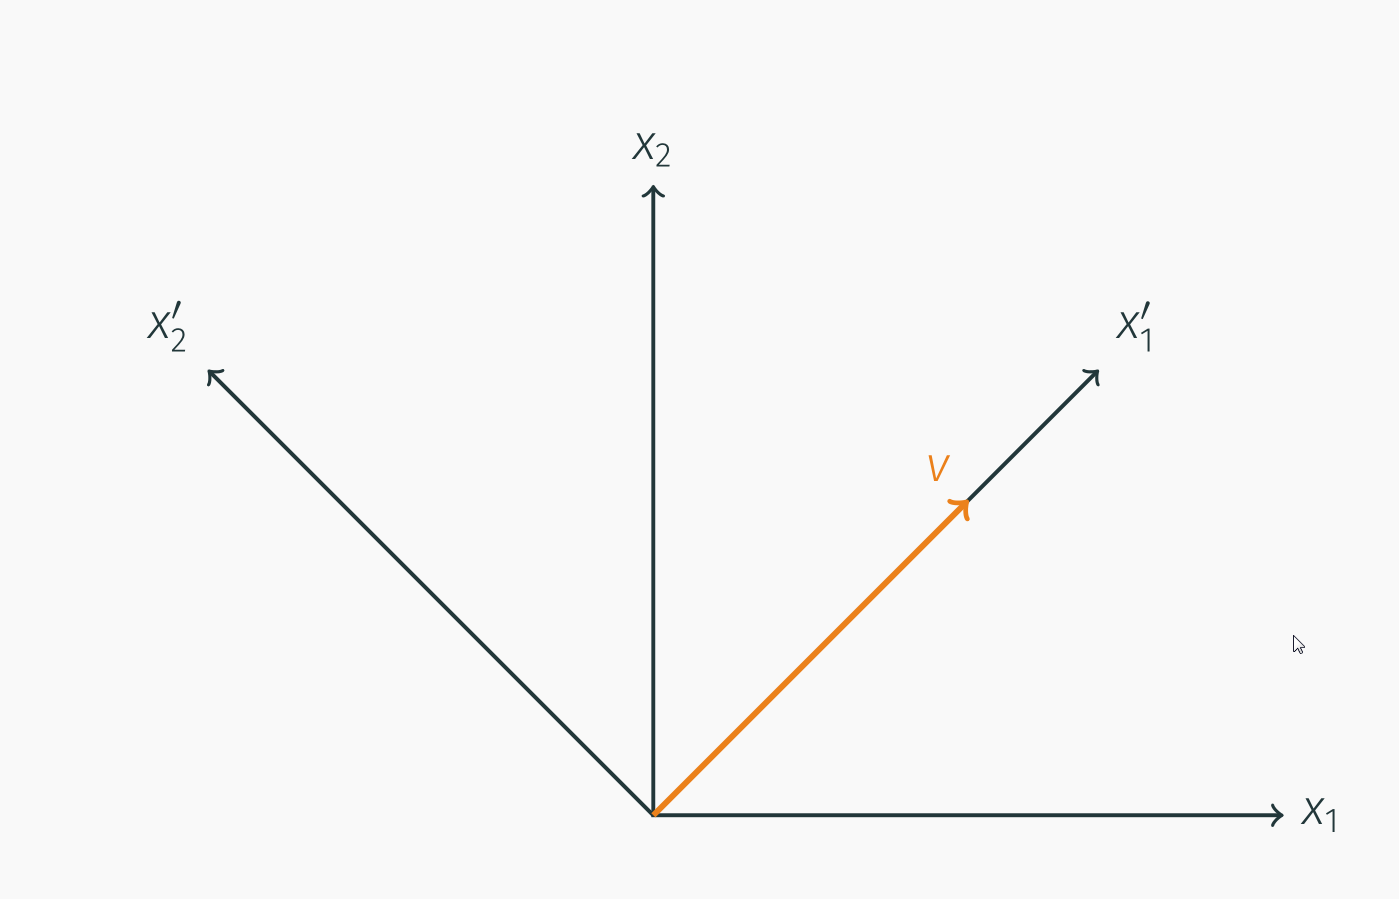
\includegraphics{../images/transform2D.png}
\end{frame}

\begin{frame}{dimensions}
\protect\hypertarget{dimensions}{}
\begin{itemize}
\tightlist
\item
  The vector, \emph{v}, remains fixed, but we transform our coordinate
  system
\item
  In the new coordinate system, the \(x_2^\prime\) portion of \emph{v}
  is zero.
\item
  To transform the coordinate system, we first define some unit vectors.
\item
  \(\hat{e}_1\) is a unit vector in the direction of \(x_1\), while
  \(\hat{e}_1^\prime\) is a unit vector in the direction of
  \(x_1^\prime\)
\end{itemize}
\end{frame}

\begin{frame}{two dimensions}
\protect\hypertarget{two-dimensions-1}{}
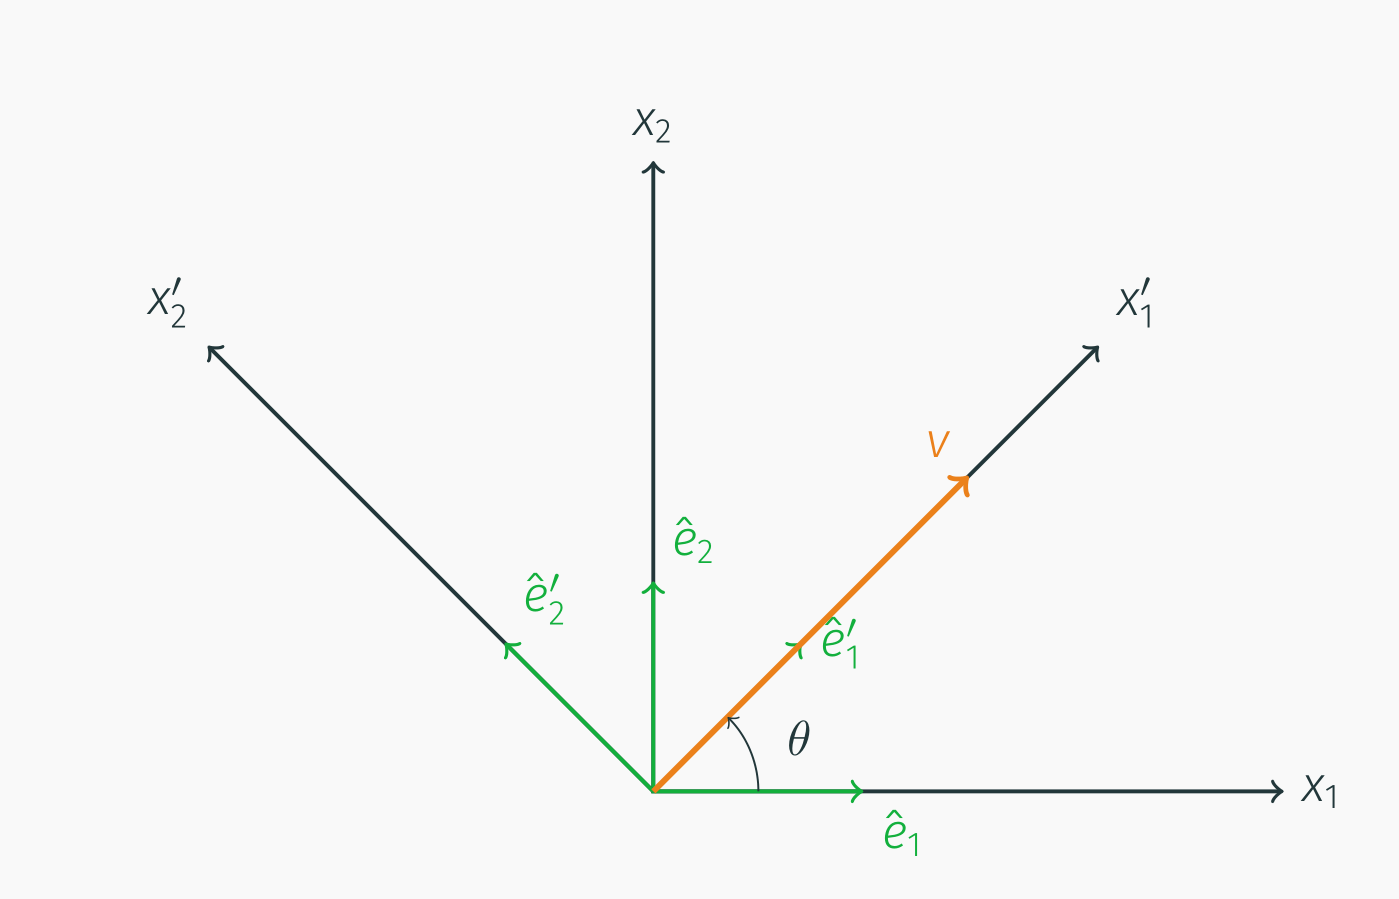
\includegraphics{../images/transform2D-unit.png}
\end{frame}

\begin{frame}{two dimensions}
\protect\hypertarget{two-dimensions-2}{}
\begin{itemize}
\tightlist
\item
  For this example, let us assume \(v = \langle 2, 2 \rangle\) and
  \(\theta = 45^\circ\)
\item
  We can write the transformed unit vectors, \(\hat{e}_1^\prime\) and
  \(\hat{e}_2^\prime\) in terms of \(\hat{e}_1\), \(\hat{e}_2\) and the
  angle of rotation, \(\theta\).
\end{itemize}

\[\begin{aligned}
\hat{e}_1^\prime &= \langle \hat{e}_1 \cos \theta , \hat{e}_2 \sin \theta\rangle\\
\hat{e}_2^\prime &= \langle -\hat{e}_1 \sin \theta , \hat{e}_2 \cos \theta \rangle\end{aligned}\]
\end{frame}

\begin{frame}{two dimensions}
\protect\hypertarget{two-dimensions-3}{}
\begin{itemize}
\tightlist
\item
  We can write the vector, \emph{v}, in terms of the unit vectors
  describing our axis system
\item
  \(v = v_1 \hat{e}_1 + v_2 \hat{e}_2\)
\item
  (note: \(\hat{e}_1=\langle 1, 0 \rangle\) and
  \(\hat{e}_2 = \langle 0,1 \rangle\) )
\item
  \(v = \langle 2, 2 \rangle = 2\langle 1, 0\rangle + 2\langle 0, 1 \rangle\)
\end{itemize}
\end{frame}

\begin{frame}{general}
\protect\hypertarget{general}{}
\begin{itemize}
\tightlist
\item
  Coordinate transformation can become much more complicated in three
  dimensions, and with higher-order tensors
\item
  It is convenient to define a general form of the coordinate
  transformation in index notation
\item
  We define \(Q_{ij}\) as the cosine of the angle between the
  \(x_i^\prime\) axis and the \(x_j\) axis.
\item
  This is also referred to as the ``direction cosine''
  \[Q_{ij} = \cos(x_i^\prime, x_j)\]
\end{itemize}
\end{frame}

\begin{frame}{general}
\protect\hypertarget{general-1}{}
\begin{itemize}
\tightlist
\item
  We can use this form on our 2D transformation example
\end{itemize}

\[\begin{aligned}
Q_{ij} &= \cos (x_i^\prime, x_j)\ &= \begin{bmatrix}
\cos (x_1^\prime, x_1) & \cos (x_1^\prime, x_2)\\
\cos (x_2^\prime, x_1) & \cos (x_2^\prime, x_2)
\end{bmatrix}\ &= \begin{bmatrix}
\cos \theta & \cos (90-\theta)\\
\cos (90+\theta) & \cos \theta
\end{bmatrix} \ &= \begin{bmatrix}
\cos \theta & \sin \theta \\
-\sin \theta & \cos \theta
\end{bmatrix}\end{aligned}\]
\end{frame}

\begin{frame}{general}
\protect\hypertarget{general-2}{}
\begin{itemize}
\tightlist
\item
  We can transform any-order tensor using \(Q_{ij}\)
\item
  Vectors (first-order tensors): \(v_i^\prime = Q_{ij}v_j\)
\item
  Matrices (second-order tensors):
  \(\sigma_{mn}^\prime = Q_{mi}Q_{nj}\sigma_{ij}\)
\item
  Fourth-order tensors:
  \(C_{ijkl}^\prime = Q_{im}Q_{jn}Q_{ko}Q_{lp}C_{mnop}\)
\end{itemize}
\end{frame}

\begin{frame}{general}
\protect\hypertarget{general-3}{}
\begin{itemize}
\tightlist
\item
  We can similarly use \(Q_{ij}\) to find tensors in the original
  coordinate system
\item
  Vectors (first-order tensors): \(v_i = Q_{ji}v_j^\prime\)
\item
  Matrices (second-order tensors):
  \(\sigma_{mn} = Q_{im}Q_{jn}\sigma_{ij}^\prime\)
\item
  Fourth-order tensors:
  \(C_{ijkl} = Q_{mi}Q_{nj}Q_{ok}Q_{pl}C_{mnop}^\prime\)
\end{itemize}
\end{frame}

\begin{frame}[fragile]{mental/emotional health warning}
\protect\hypertarget{mentalemotional-health-warning}{}
\begin{itemize}
\item
\begin{verbatim}
  Some texts flip the definition of \\(Q_{ij}\\), and then flip their transformation law accordingly
\end{verbatim}
\item
\begin{verbatim}
  Any time you use tensor transformation, make sure you are following a consistent set of transformation laws
\end{verbatim}
\end{itemize}
\end{frame}

\begin{frame}{general}
\protect\hypertarget{general-4}{}
\begin{itemize}
\tightlist
\item
  We can derive some interesting properties of the transformation
  tensor, \(Q_{ij}\)
\item
  We know that \(v_i = Q_{ji}v_j^\prime\) and that
  \(v_i^\prime = Q_{ij}v_j\)
\item
  If we substitute (changing the appropriate indexes) we find:
\item
  \(v_i = Q_{ji}Q_{jk}v_k\)
\item
  We can now use the Kronecker Delta to substitute
  \(v_i = \delta_{ik}v_k\) which gives
\item
  \(\delta_{ik}v_k} = Q_{ji}Q_{jk}v_k\)
\end{itemize}
\end{frame}

\hypertarget{examples}{%
\section{examples}\label{examples}}

\begin{frame}{example}
\protect\hypertarget{example-5}{}
\begin{columns}[T]
\begin{column}{0.5\textwidth}
\begin{figure}
\centering
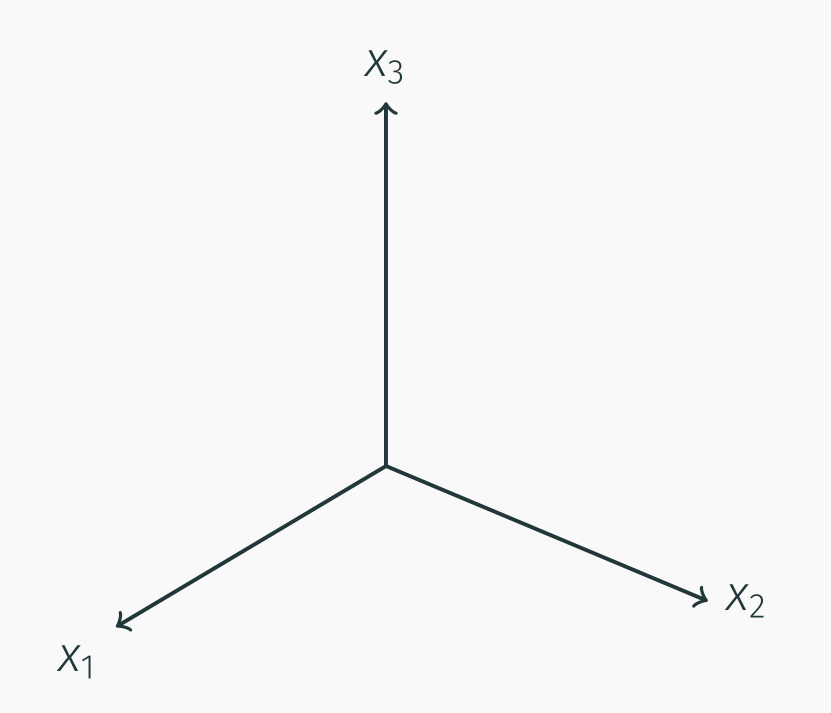
\includegraphics{../images/example-a.png}
\caption{empty 3D coordinate system with axes labeled for example
problem}
\end{figure}
\end{column}

\begin{column}{0.5\textwidth}
\begin{itemize}
\tightlist
\item
  Find \(Q_{ij}^1\) for rotation of \(60^\circ\) about \(x_2\)
\item
  Find \(Q_{ij}^2\) for rotation of \(30^\circ\) about \(x_3^\prime\)
\item
  Find \(e_i^{\prime \prime}\) after both rotations
\end{itemize}
\end{column}
\end{columns}
\end{frame}

\begin{frame}{example}
\protect\hypertarget{example-6}{}
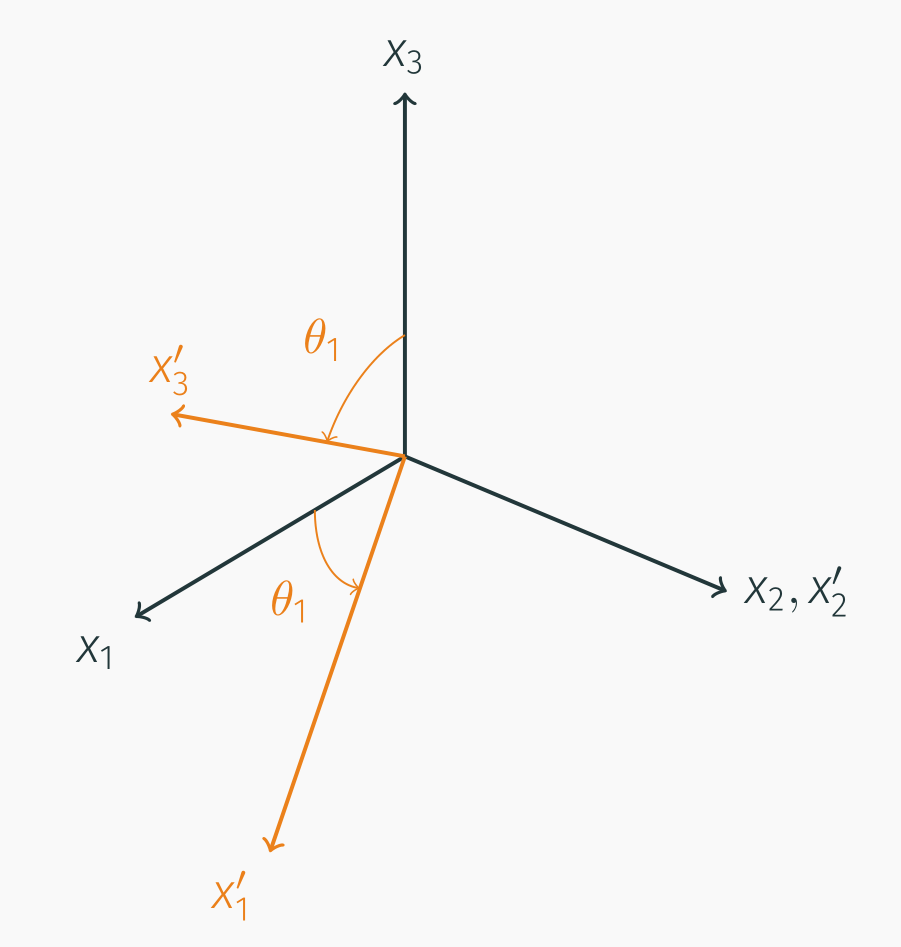
\includegraphics{../images/example-b.png}
\end{frame}

\begin{frame}{example}
\protect\hypertarget{example-7}{}
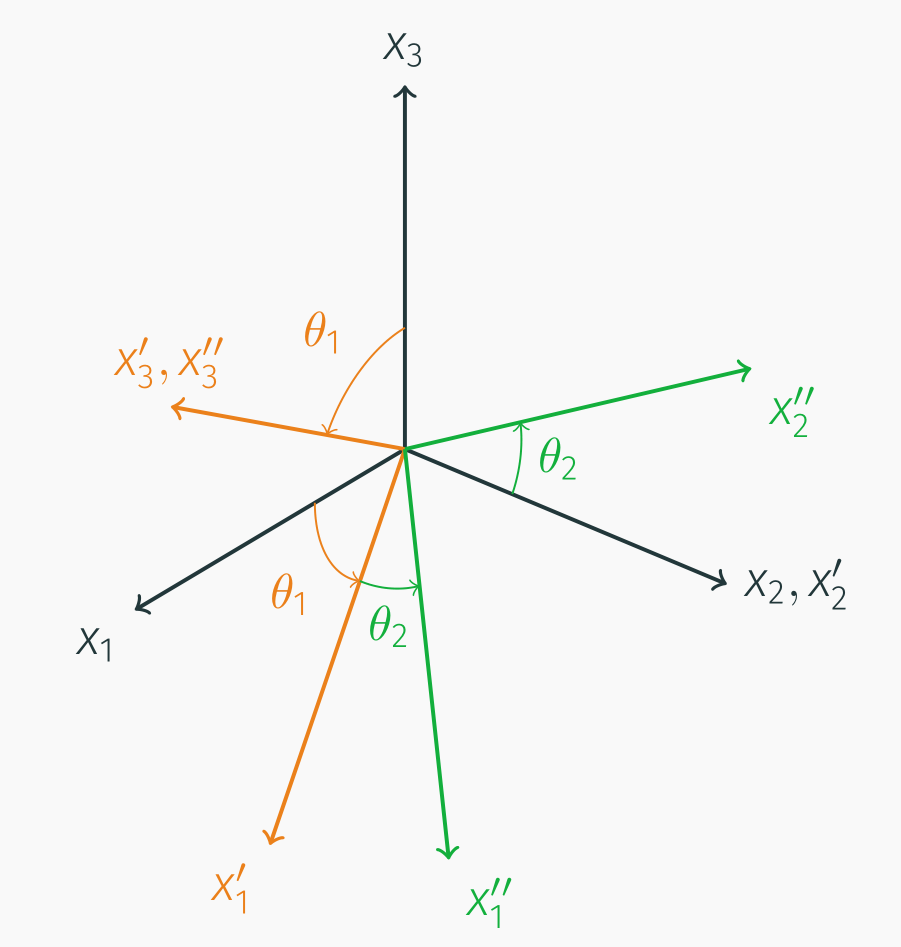
\includegraphics{../images/example-c.png}
\end{frame}

\begin{frame}{example}
\protect\hypertarget{example-8}{}
\begin{itemize}
\tightlist
\item
  \(Q_{ij}^1 = \cos(x_i^\prime, x_j)\)
\item
  \(Q_{ij}^2 = \cos(x_i^\prime, x_j)\)
\end{itemize}

\[Q_{ij}^1 = \begin{bmatrix}
\cos 60 & \cos 90 & \cos 150\\
\cos 90 & \cos 0 & \cos 90\\
\cos 30 & \cos 90 & \cos 60
\end{bmatrix}\] \[Q_{ij}^2 = \begin{bmatrix}
\cos 30 & \cos 60 & \cos 90\\
\cos 120 & \cos 30 & \cos 90\\
\cos 90 & \cos 90 & \cos 0
\end{bmatrix}\]
\end{frame}

\begin{frame}{example}
\protect\hypertarget{example-9}{}
\begin{itemize}
\tightlist
\item
  We now use \(Q_{ij}\) to find \(\hat{e}_i^\prime\) and
  \(\hat{e}_i^{\prime \prime}\)
\item
  First, we need to write \(\hat{e}_i\) in a manner more consistent with
  index notation
\item
  We will indicate axis direction with a superscript,
  e.g.~\(\hat{e}_1 = e_i^1\)
\item
  \(e_i^\prime = Q_{ij}^1 e_j\)
\item
  \(e_i^{\prime \prime} = Q_{ij}^2 e_j^\prime\)
\item
  How do we find \(e_i^{\prime \prime}\) in terms of \(e_i\)?
\item
  \(e_i^{\prime \prime} = Q_{ij}^2 Q_{jk}^1 e_k\)
\end{itemize}
\end{frame}

\end{document}
